\documentclass{beamer}

\usepackage[utf8]{inputenc}
\usepackage{minted} %Allow synthax highlit on code snippets
\usepackage{xcolor}
\usetheme{CambridgeUS}

\title{Introduction to the iPOP-UP HPC cluster}
\author[Rey, Kirsh and Hennion]{Julien Rey \and Olivier Kirsh \and Magali Hennion}
\date{Juin 2023}



\logo { 
    
\includegraphics[height=1cm]{Logo/ipopup.png}
}


%\logo{
%    
\includegraphics[width=1cm]{Logo/ipopup.png}
%}

\titlegraphic{
    
\includegraphics[height=1.5cm]{Logo/ipopup.png}
    \hspace{1cm}
    
\includegraphics[height=1.5cm]{Logo/UniversiteLogo.png}
    \hspace{1cm}
    
\includegraphics[height=1.5cm]{Logo/RPBS.png}
}


\begin{document}
{
\setbeamertemplate{logo}{}
\begin{frame}
    \maketitle
\end{frame}
}

\begin{frame}
\frametitle{Table of Contents}
\tableofcontents
\end{frame}

\section{Introduction}
\begin{frame}[fragile]{Who is this training for}
    \begin{itemize}
        \item You work at Université Paris Cité
        \item You need (or might need) more computational power than you currently have
        \item You are familiar with Unix systems and Bash
    \end{itemize}
\end{frame}

\section{The RPBS platform}
\begin{frame}[fragile]{Missions}
    \begin{center}
        
\includegraphics[height = 1.5cm]{Logo/RPBS.png}
    \end{center}
    \begin{itemize}
        \item Development of Structural Bioinformatics methods
        \item Services deployment on the computing resource
        \item Expertise and training
        \item Hardware hosting
    \end{itemize}
\end{frame}

\begin{frame}[fragile]{Web portal}
\begin{columns}
    \begin{column}{0.7\textwidth}
        \begin{itemize}
            \item https://mobyle.rpbs.univ-paris-diderot.fr: free access
            \item 30+ Structural Bioinformatics services
            \item ~1 million CPU hours /year
            \item ~80,000 jobs /year
        \end{itemize}
    \end{column}
    \begin{column}{0.3\textwidth}
        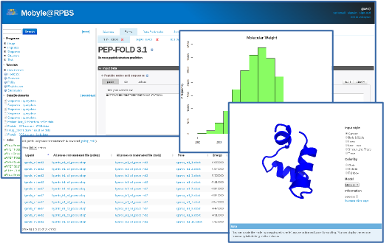
\includegraphics[height = 2cm]{Images/mobyle.png}
    \end{column}
\end{columns}
\begin{columns}
    \begin{column}{0.5\textwidth}
        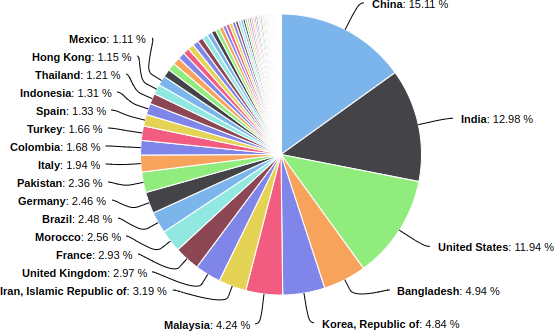
\includegraphics[height = 3cm]{Images/country2022.png}
    \end{column}
    \begin{column}{0.5\textwidth}
        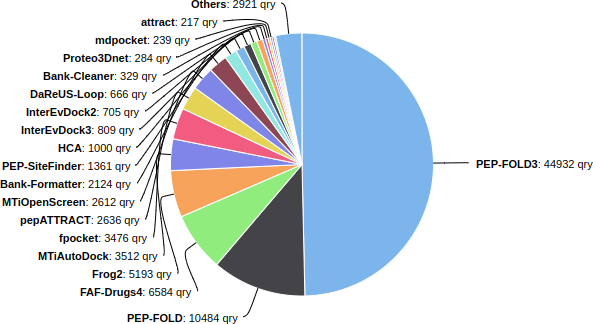
\includegraphics[height = 3cm]{Images/service2022.png}
    \end{column}
\end{columns}
\end{frame}

\begin{frame}[fragile]{The iPOP-UP project}
\begin{center}
    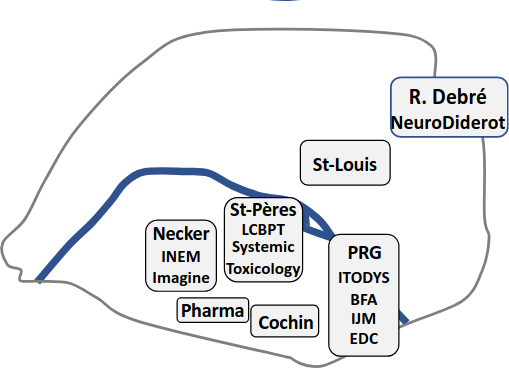
\includegraphics[height = 3cm]{Images/multisite.png}   
\end{center}
\begin{itemize}
    \item iPOP-UP: \underline{I}ntegrative \underline{P}latform for \underline{O}mics \underline{P}rojects at \underline{U}niversité de \underline{P}aris
    \item Multisite Bioinformatics platform
    \item Ranging from multiple 'Omics' techniques to structural and chemo- \emph{in silico} Bioinformatics
    \item Compute nodes
\end{itemize}
\end{frame}

\section{Cluster description}
\begin{frame}{What is a cluster for ?}
    \begin{itemize}
        \item High hardware resources needs
        \item Long running analyses
        \item A lot of similar analyses
        \item Shared work between users
        \item Free your desktop from the task
    \end{itemize}
\end{frame}


\begin{frame}{What is a cluster ?}
\centering
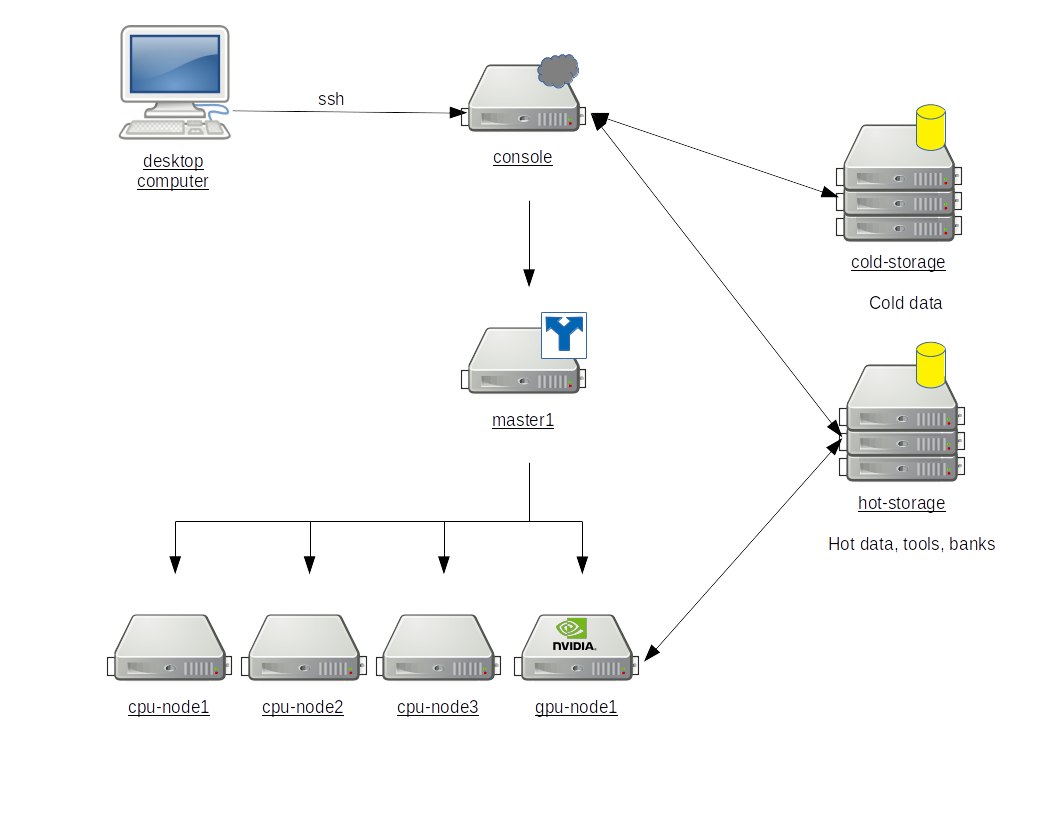
\includegraphics[keepaspectratio=True, width =0.9\textwidth]{Images/architecture.png}
\end{frame}

\begin{frame}{Computational hardware}
Partitions (groups of compute nodes):
\begin{itemize}
    \item ipop-up: 16 nodes, 2048 CPUs
    \item rpbs: 20 nodes, 832 CPUs, 9 GPUs (+ 9 nodes, 520 CPUs, 4 GPUs)
    \item cmpli: 6 nodes, 264 CPUs, 14 GPUs (+ 1 node, 64 CPUs, 2 GPUs)
    \item epigen: 4 nodes, 128 CPUs
    \item master-bi: 1 node, 32 CPUs, 3 GPUs
\end{itemize}
Storage:
\begin{itemize}
    \item hot-storage: 125TB, very fast
    \item cold-storage: 240TB, slow + backup (soon)
\end{itemize}

\end{frame}

\begin{frame}[fragile]{In practice}
Go to your terminal and connect to the cluster using the following line, don't forget to replace username with your personal username.
\begin{minted}[bgcolor=lightgray]{bash}
ssh username@ipop-up.rpbs.univ-paris-diderot.fr
\end{minted}
Type in your password and  enter. 
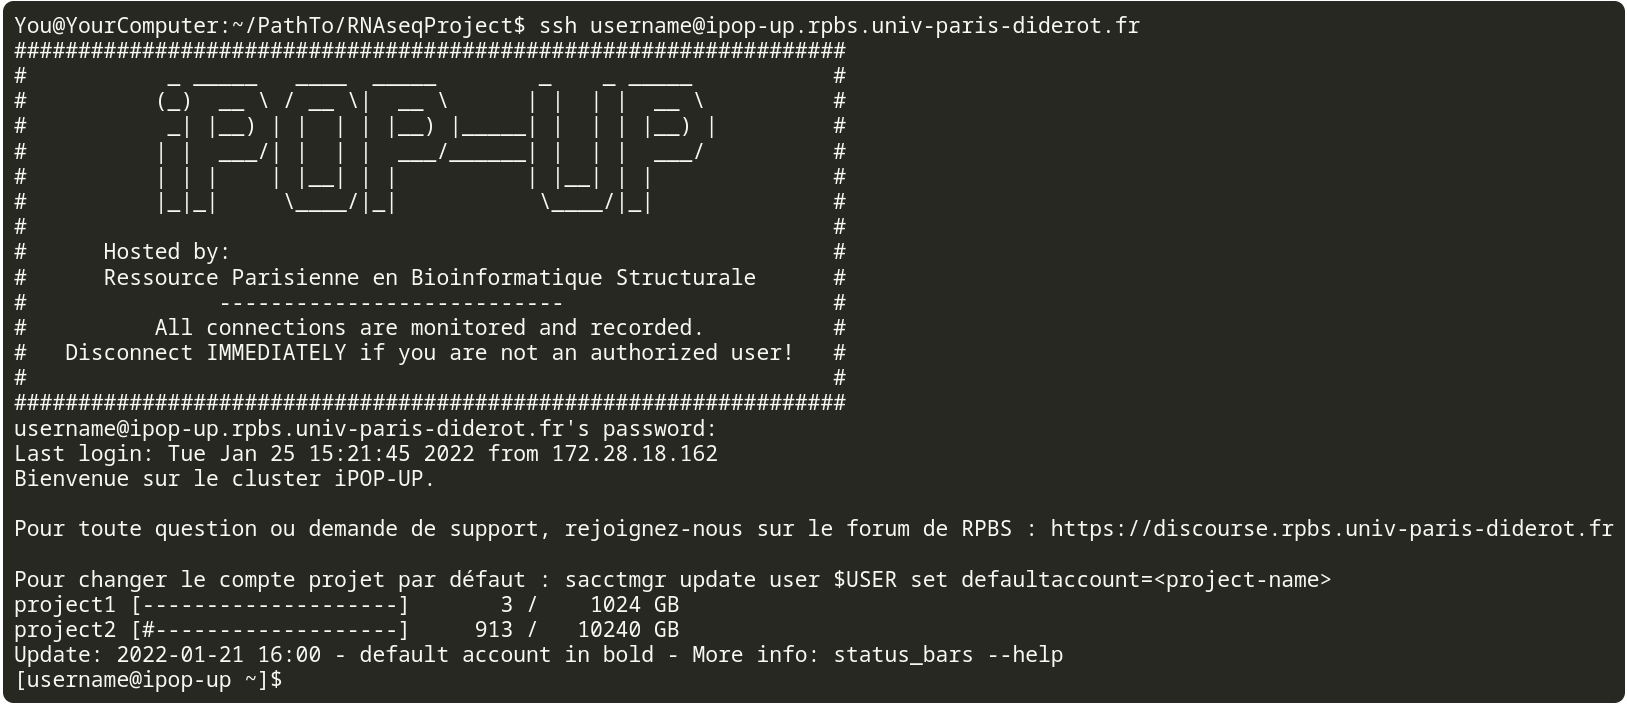
\includegraphics[keepaspectratio=True, height=4cm]{Images/connexionCluster.png}
\end{frame}

\begin{frame}[fragile]{Note about ssh and security}
Your IP will be banned after 5 failed authentication attempts. Each public keys count as one authentication attempt. To disable public key authentication:
\begin{minted}[bgcolor=lightgray,breaklines]{bash}
ssh -o PubkeyAuthentication=no username@ipop-up.rpbs.univ-paris-diderot.fr
\end{minted}
A good thing to do, change your password:   
\begin{minted}[bgcolor=lightgray]{bash}
passwd
\end{minted}

\end{frame}

\section{Cluster's basics}
\begin{frame}[fragile]{Where you can go, write, or execute}
\begin{block}{User environments}
\begin{minted}{bash}
/shared/home/username
\end{minted}
\end{block}

\begin{block}{Computations (hot data)}
\begin{minted}{bash}
/shared/projects/projectname
\end{minted}
\end{block}

\begin{block}{Processed data (cold data)}
\begin{minted}{bash}
/cold-storage/username
\end{minted}
\end{block}

\begin{block}{Data banks (read-only)}
\begin{minted}{bash}
/shared/banks/
\end{minted}
\end{block}
\end{frame}

\begin{frame}[fragile]{Slurm}


\includegraphics[height = 1cm]{Logo/Slurm.png} \\
Slurm is the cluster management and job scheduling system.\\

It is what will take your code and distribute it on one of the computing nodes, while ensuring it has the CPU(s) and RAM that you asked for.
\\

It requires specific commands to run (srun, sbatch, salloc, etc...)
\end{frame}

\begin{frame}{What is a cluster ?}
\centering
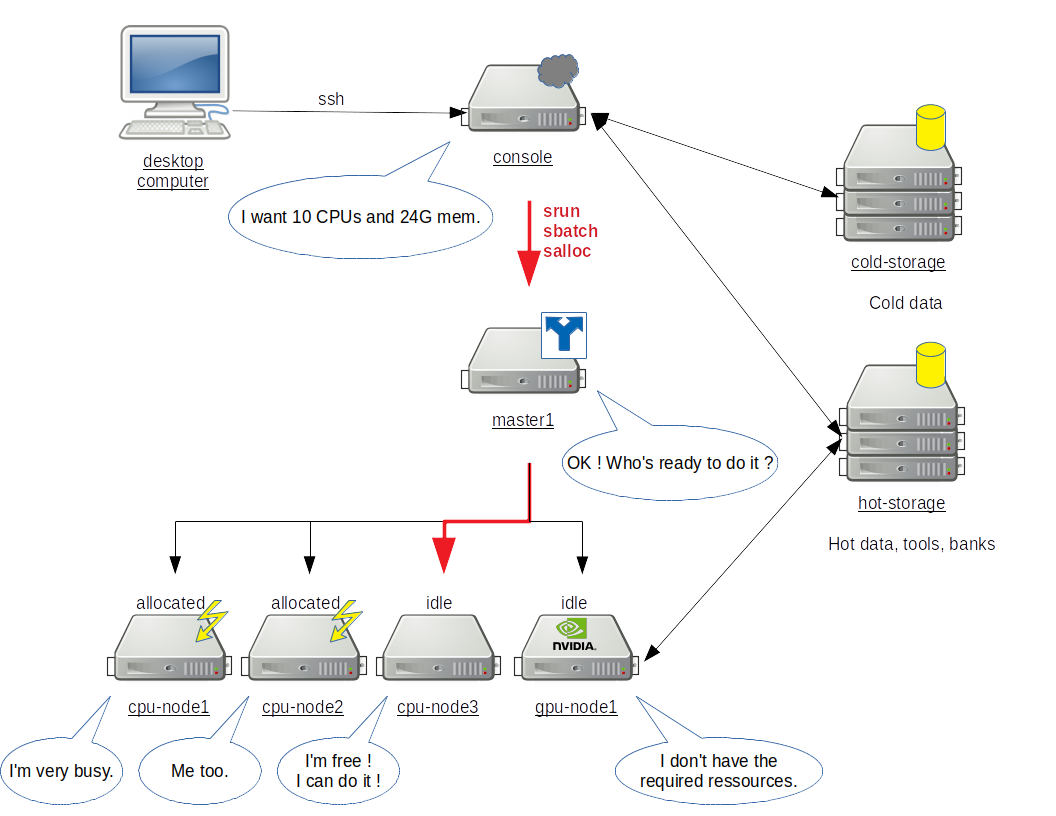
\includegraphics[keepaspectratio=True, width =0.9\textwidth]{Images/slurm_submit.png}
\end{frame}

\begin{frame}[fragile]{Modules}
A lot of tools are installed on the cluster.
\\

\begin{block}{To list them}
    \verb|module available| \\
    \verb|module av|
\end{block}

 
\begin{block}{For example}
    Look for the different versions of multiqc on the cluster using \verb|module av multiqc|
\end{block}
\begin{center}
    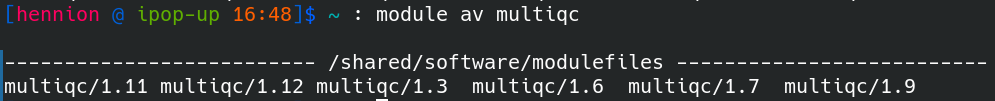
\includegraphics[height = 1cm]{Images/multiqc.png}
\end{center}
\end{frame}

\begin{frame}[fragile]{Modules}
    \begin{columns}
    \begin{column}{0.4\textwidth}
    \textbf{To load a tool}
    \verb|module load tool/1.3|
    \verb|module load tool1 tool2 tool3|
   
    \end{column}
    \begin{column}{0.1\textwidth}
    \\
    \end{column}
    \begin{column}{0.4\textwidth}
    \textbf{To list modules loaded}\\
    \verb|module list|
    \\
    \parskip=8pt
    \textbf{To remove all loaded modules}\\
    \verb|module purge|
    \end{column}
    \end{columns}
    \parskip=20pt
    \begin{center}
        \textbf{Load your modules within your "sbatch" file for consistency}
    \end{center}
\end{frame}



\begin{frame}[fragile]{Job monitoring - squeue}
On your terminal, type \verb|squeue|
\begin{center}
    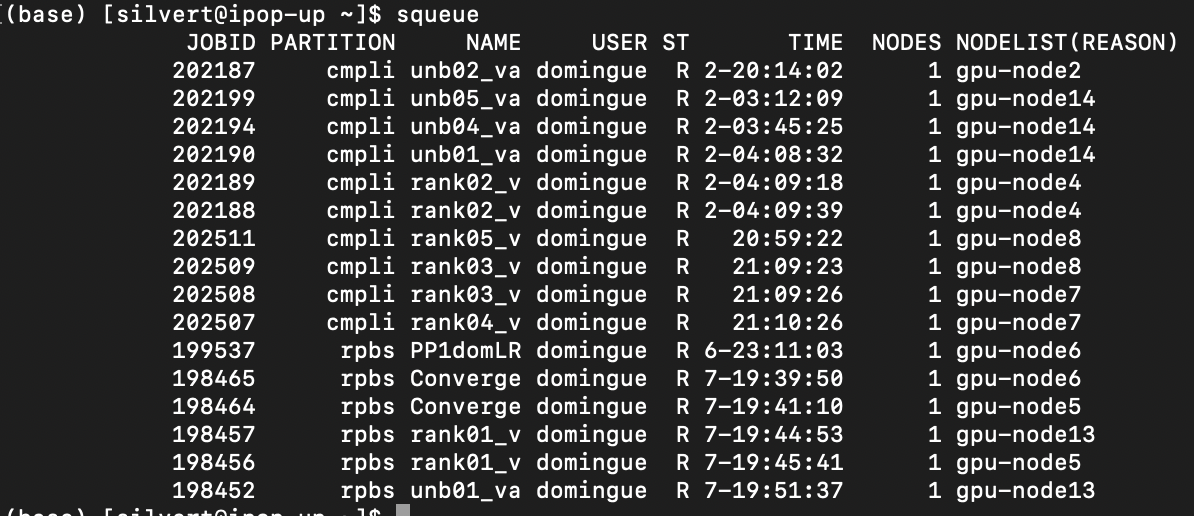
\includegraphics[height = 3.5cm]{Images/squeue.png}
\end{center}

ST : Status of the job. R means Running, PD means Pending\\
\begin{columns}
\begin{column}{5cm}
To see only iPOP-UP jobs
\verb|squeue -p ipop-up|
\end{column}

\begin{column}{5cm}
To see only your jobs
\verb|squeue -u username|
\end{column}
\end{columns}
\end{frame}
    
    



\begin{frame}[fragile]{Monitoring your jobs, sacct}
(Re-run sleep if needed and) type \verb|sacct| 
    
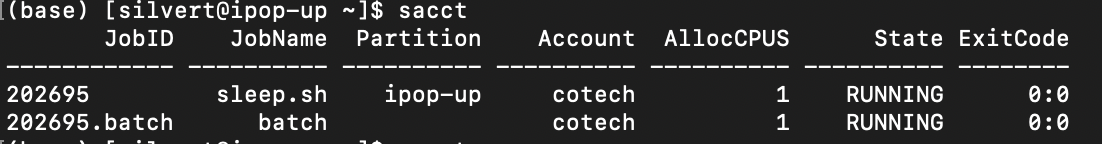
\includegraphics[height = 1.5cm]{Images/sacct.png}

\parskip=12pt

You can pass the option \verb|--format| to list the information that you want to display, including memory usage, time of running, ... For instance: \\
\verb|sacct --format=JobID,JobName,Start,Elapsed,CPUTime,|  \\
\verb|NCPUS,NodeList,MaxRSS,ReqMeM,State|
\parskip=12pt

To see every options, run \verb|sacct --helpformat|

\end{frame} 

\begin{frame}[fragile]{Job efficiency}
    After the run, the \verb|seff| command allows you to access information about the efficiency of a job.
    
    \verb|seff <jobid>|
    \begin{center}
            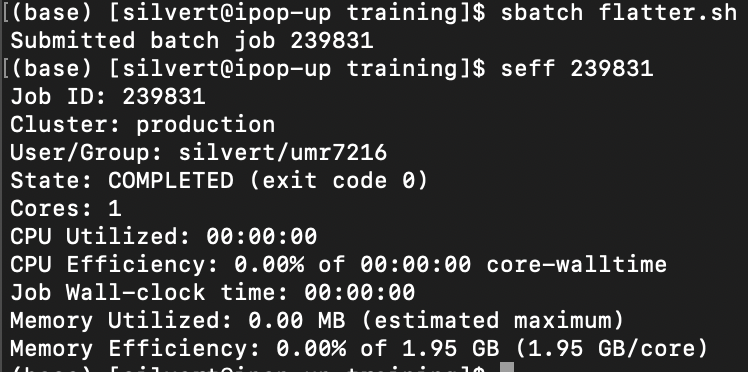
\includegraphics[width = 8cm]{Images/seffExample.png}
    \end{center}

Exercices star etc...
   
\end{frame}

\section{Parallelization}
\begin{frame}[fragile]{Some vocabulary}
\begin{itemize}
    \item job : A script, typically started with sbatch
    \item job step : A specific step in the big job, it can be a "srun" line within the script
    \item job task : A unit of resource allocation
\end{itemize}

We will not go into \verb|srun| usage here, but we can talk about it later if you want.
%If you do not use \verb|srun| \textbf{cpus-per-task corresponds to the number of CPUs asked.}  % je comprends pas la phrase!! 
    
\end{frame}


\begin{frame}[fragile]{Ask for more CPUs for a tool}

Some tools allow multi-threading, i.e. the use of several CPUs to accelerate one task. \\
It is the case of STAR with the \verb|--runThreadN| option. 

\begin{block}{Exercise : Alignment, parallel}
\end{block}

\end{frame}

\begin{frame}{The cost of parallelization}
\begin{itemize}
    \item It may cost more in memory
    \item The gain in time is not linear
\end{itemize}
\end{frame}

\begin{frame}[fragile]{Job arrays}
Job arrays allow to start the same job a lot of times (same executable, same resources)

\vspace{10pt}

\begin{minted}[fontsize=\small]{bash}
#SBATCH --array=0-3
\end{minted}

Slurm variables

\$SLURM\_ARRAY\_JOB\_ID

\$SLURM\_ARRAY\_TASK\_ID


\end{frame}


\begin{frame}[fragile]{Job Array Common Mistakes}
\begin{itemize}
    \item The index of bash lists starts at 0
    \item Don't forget to have different output files for each task of the array
    \item Same with your log names (\%a or \%J in the name will do the trick)
    \item Do not overload the cluster! Please use \%50 (for example) at the end of your indexes to limit the number of tasks (here to 50) running at the same time. The 51st will start as soon as one finishes!
    \item The RAM defined using \verb|#SBATCH --mem=25G| is for each task
\end{itemize}
    
\end{frame}

\begin{frame}[fragile]{Complex workflows}
\begin{center}
    
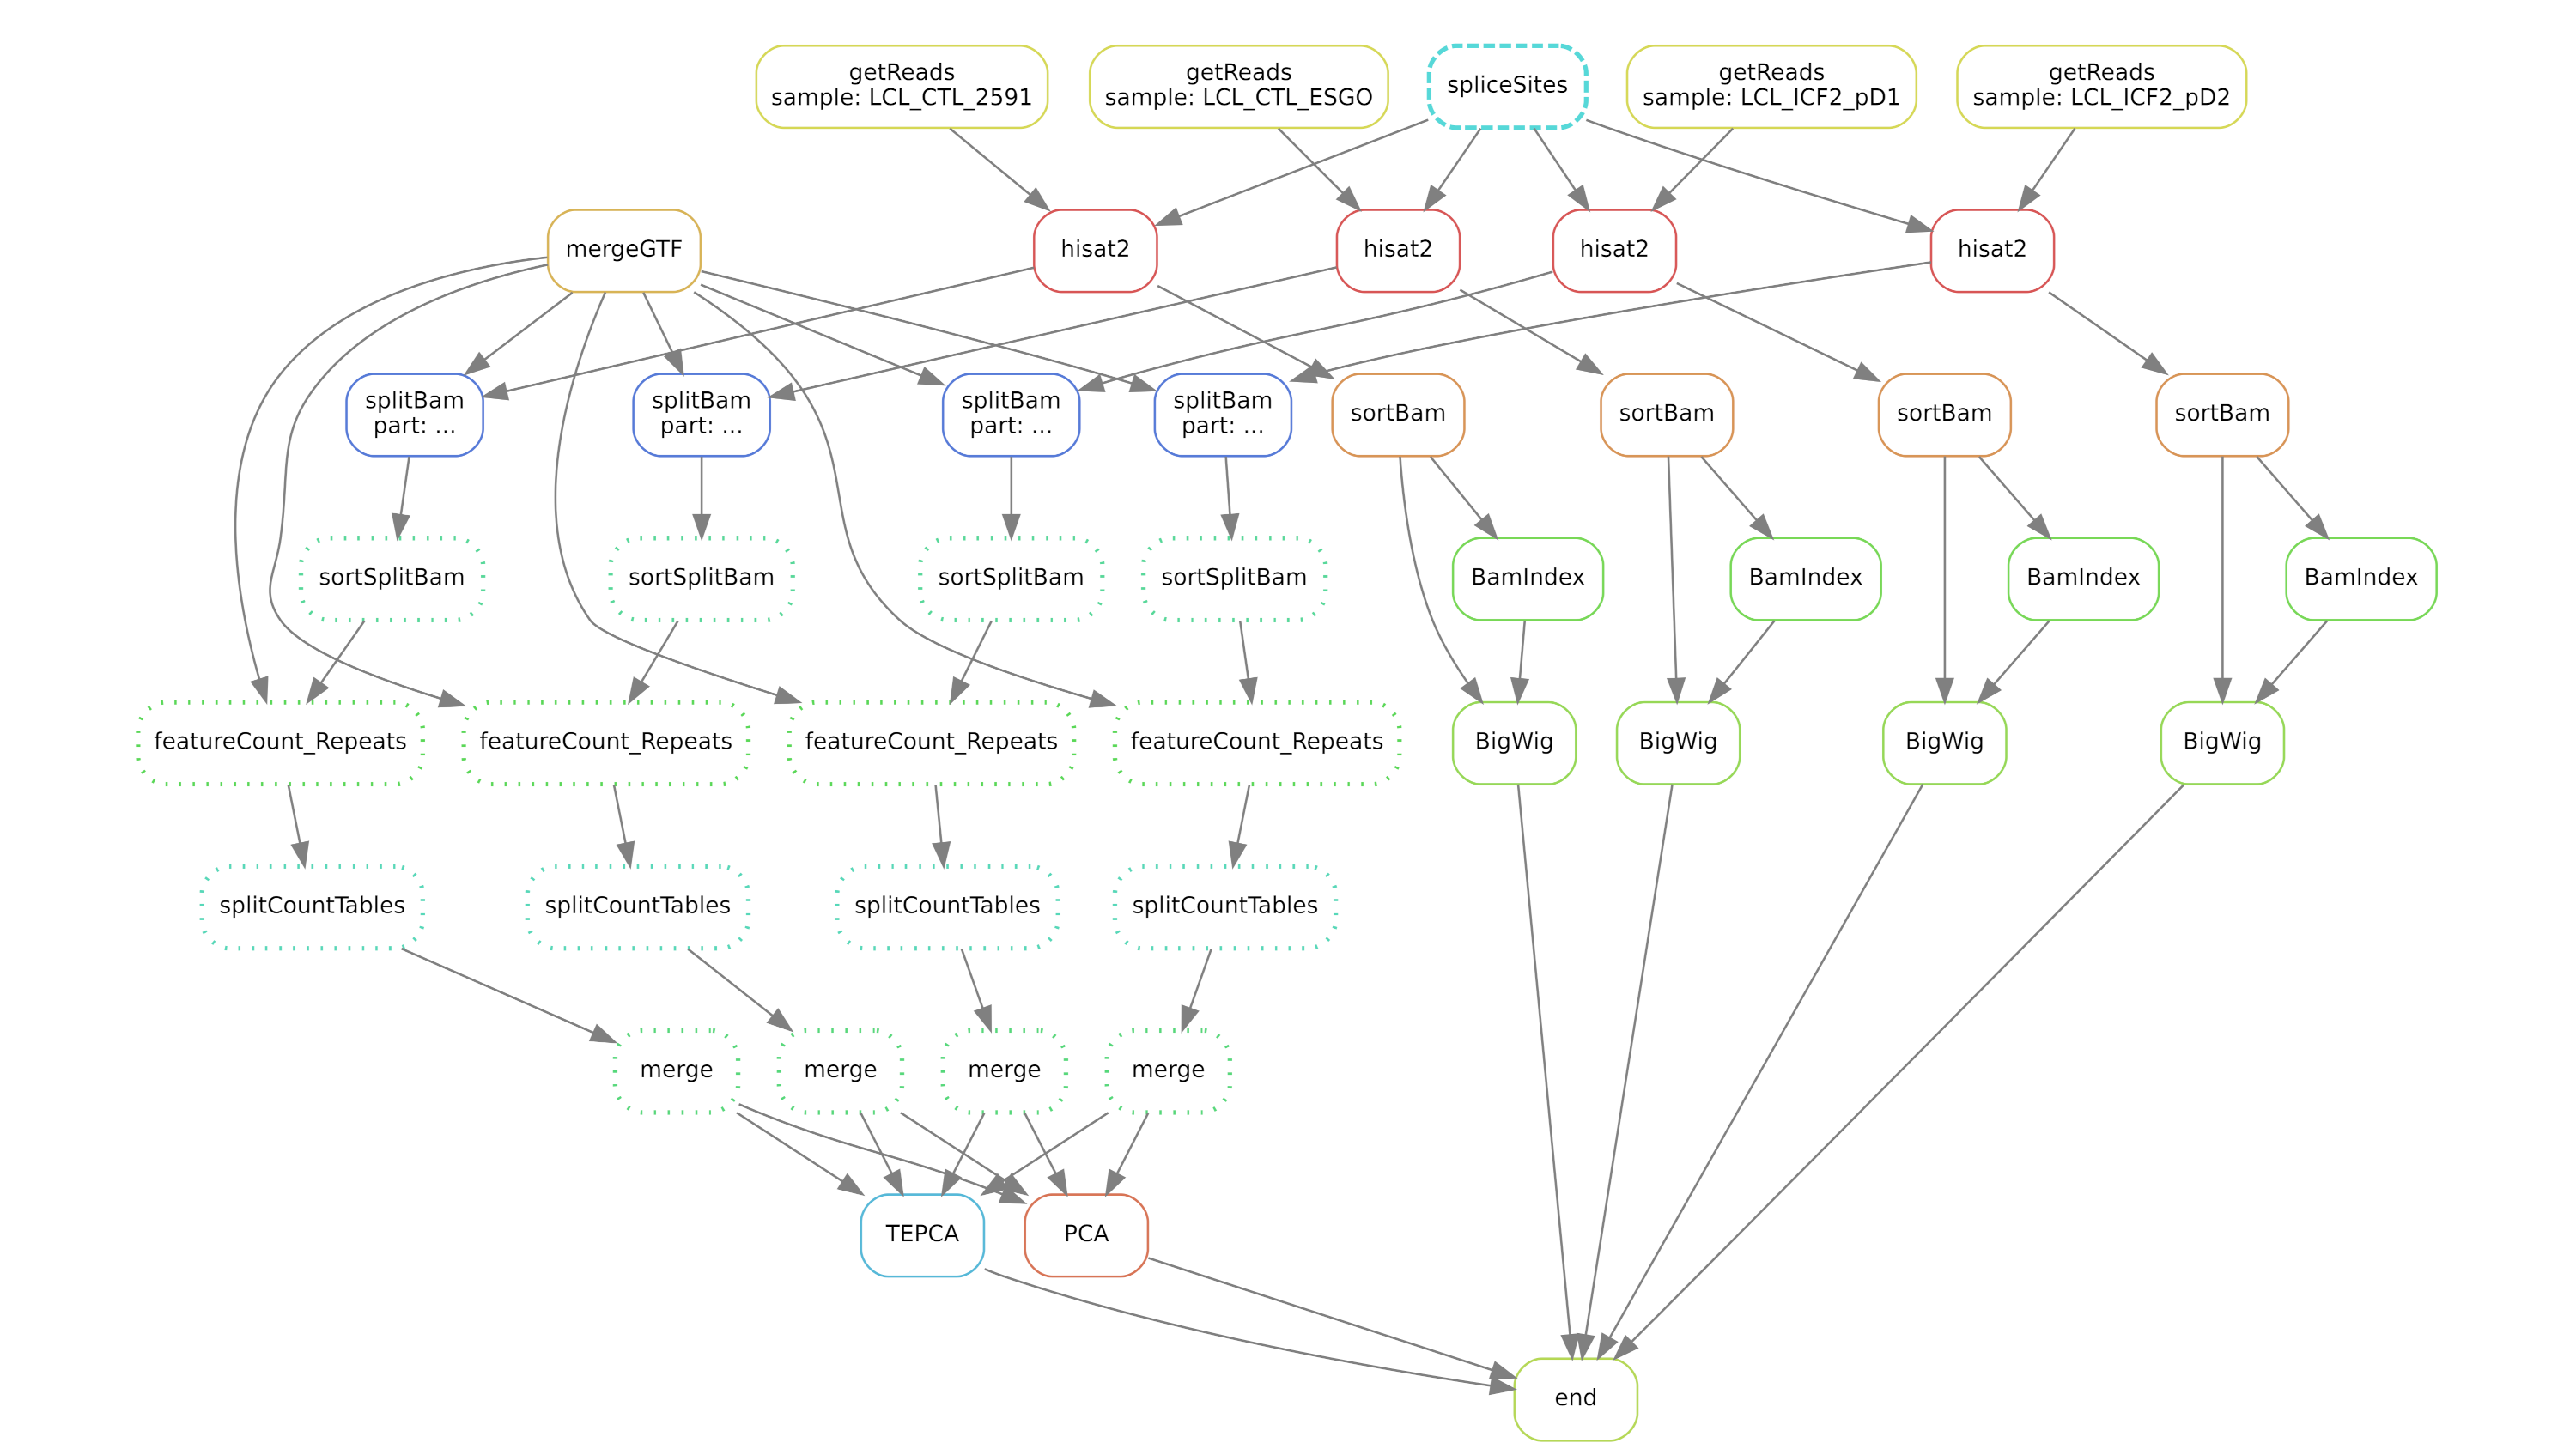
\includegraphics[height = 6cm]{Images/snakemake.png} \\
\end{center}

Use workflow managers such as Snakemake or Nextflow. 
    
\end{frame}

\section{Useful resources}
\begin{frame}[fragile]{Useful resources}

    To find out more, the SLURM manual : \verb|man sbatch| or \href{https://slurm.schedmd.com/sbatch.html}{https://slurm.schedmd.com/sbatch.html} \\
    
    
    Ask for help or signal problems on the cluster : \href{https://discourse.rpbs.univ-paris-diderot.fr/}{https://discourse.rpbs.univ-paris-diderot.fr/} \\

    iPOP-UP cluster documentation: \\
    \href{https://ipop-up.docs.rpbs.univ-paris-diderot.fr/documentation/}
    {https://ipop-up.docs.rpbs.univ-paris-diderot.fr/documentation/}
    
\end{frame}

\section{Ending}
\begin{frame}{Thanks}
    \center
    
\includegraphics[height=1.5cm]{Logo/RPBS.png}
    \hspace{1cm}
    
\includegraphics[height=1.5cm]{Logo/UniversiteLogo.png}
    \vspace{1cm}
    \begin{columns}
    \begin{column}{0.4\textwidth}
    \end{column}
   \begin{column}{0.4\textwidth}
    iPOP-UP's technical and steering comitees

    \end{column}
\end{columns}
\end{frame}


\end{document}
